\chapter{Dataset Analysis}
\label{ch:dataset}

\section{KVP10k Dataset}
\label{sec:kvp10k}

The KVP10k dataset \cite{kvp10k} is a large-scale benchmark for \kvp{} extraction from business documents. It consists of 48,280 training samples and 5,255 test samples, spanning diverse document types including invoices, forms, and receipts.

\subsection{Data Collection and Annotation Format}
The dataset was collected by IBM Research from real-world business documents, with manual annotation of bounding boxes and key-value relationships. Each sample consists of a document scan or photo together with a list of annotations. Every annotation carries a set of polygon \texttt{coordinates} (a list of $\{x, y\}$ points), a \texttt{label} giving its type (for example Text or identifier), and an \texttt{attributes.Linking} field that references the identifier of the annotation it is linked to, thereby encoding the key--value relationship.

\section{Layout Clustering Analysis}
\label{sec:layout_clustering}

We perform unsupervised clustering to identify recurring document layout types in the dataset. This provides a compact way to stratify evaluation in later stages and to check whether model performance varies across layout regimes.

\subsection{Feature Extraction}
\label{subsec:features}

We extract 13 layout features per document (see Table \ref{tab:features}):

\begin{table}[h]
\centering
\caption{Layout features extracted from each document}
\label{tab:features}
\begin{tabular}{@{}ll@{}}
\toprule
\textbf{Feature} & \textbf{Description} \\ \midrule
$n_{\text{boxes}}$ & Number of bounding boxes \\
$A_{\text{total}}$ & Total area covered by boxes \\
$\mu_A$ & Mean box area \\
$\sigma_A$ & Standard deviation of box area \\
$\mu_w$ & Mean box width \\
$\mu_h$ & Mean box height \\
$\mu_r$ & Mean aspect ratio (width/height) \\
$\mu_x$ & Mean x-position (horizontal center) \\
$\mu_y$ & Mean y-position (vertical center) \\
$\rho$ & Layout density (total coverage) \\
$s_v$ & Vertical spread (max$_y$ - min$_y$) \\
$s_h$ & Horizontal spread (max$_x$ - min$_x$) \\
$d_{\text{spacing}}$ & Mean inter-box Euclidean distance \\ \bottomrule
\end{tabular}
\end{table}

\subsection{K-means Clustering}
\label{subsec:kmeans}

We apply K-means clustering \cite{kmeans} on standardized layout features. To select the number of clusters, we sweep $k \in \{2,\dots,10\}$ and evaluate multiple complementary criteria: (i) Silhouette score (primary), (ii) Davies--Bouldin index, (iii) Calinski--Harabasz score, and (iv) the inertia curve (elbow). We use a fixed random seed and standardization to make the selection reproducible.

Figures~\ref{fig:stage2_optimal_k} and~\ref{fig:stage2_cluster_dist} summarize the selection outcome. Across the considered range, the criteria consistently favor a small number of well-separated clusters. In particular, the silhouette score peaks at \textbf{0.763} for $k=2$ (0.7627), and we therefore choose \textbf{$k=2$}.

\textbf{Results:} Two distinct layout types were identified on the annotated KVP10k training pages ($n=25{,}692$). This analysis covers the filtered subset of pages with a usable text layer: during preparation, PyMuPDF retained only pages from which text and bounding boxes could be extracted, and pages without a text layer (e.g.\ purely scanned images) were dropped. The clustering therefore separates pages by the density of \emph{extractable} text rather than by document genre:

\begin{figure}[H]
    \centering
    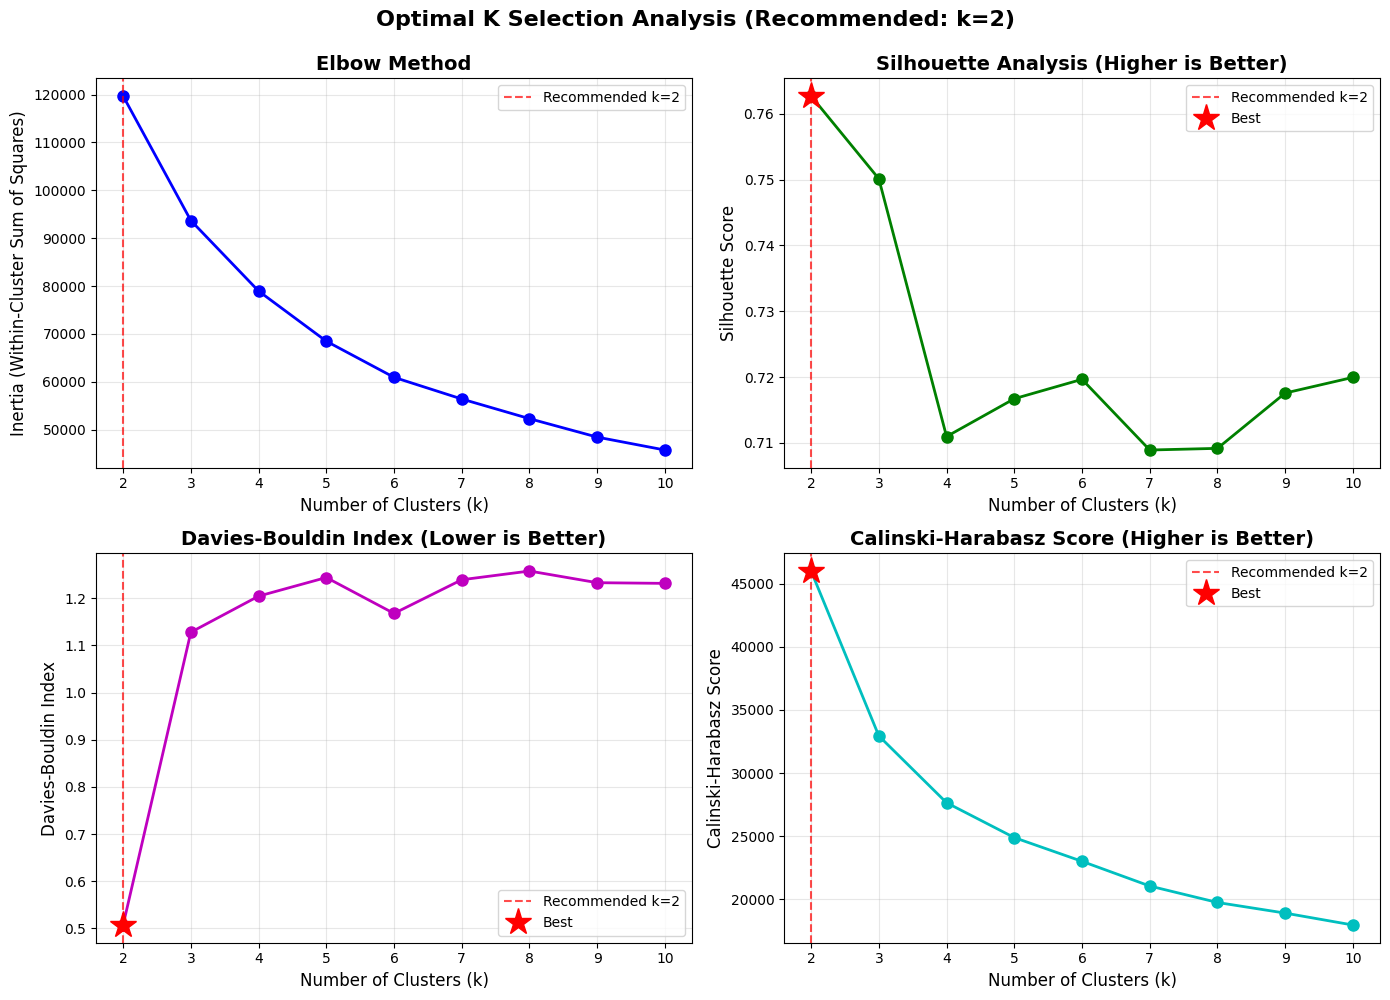
\includegraphics[width=0.75\textwidth]{figures/stage2/optimal_k_analysis.png}
    \caption{Stage 2 layout clustering: optimal $k$ selection across multiple criteria (silhouette, Davies--Bouldin, Calinski--Harabasz, and the inertia elbow).}
    \label{fig:stage2_optimal_k}
\end{figure}

\begin{figure}[H]
    \centering
    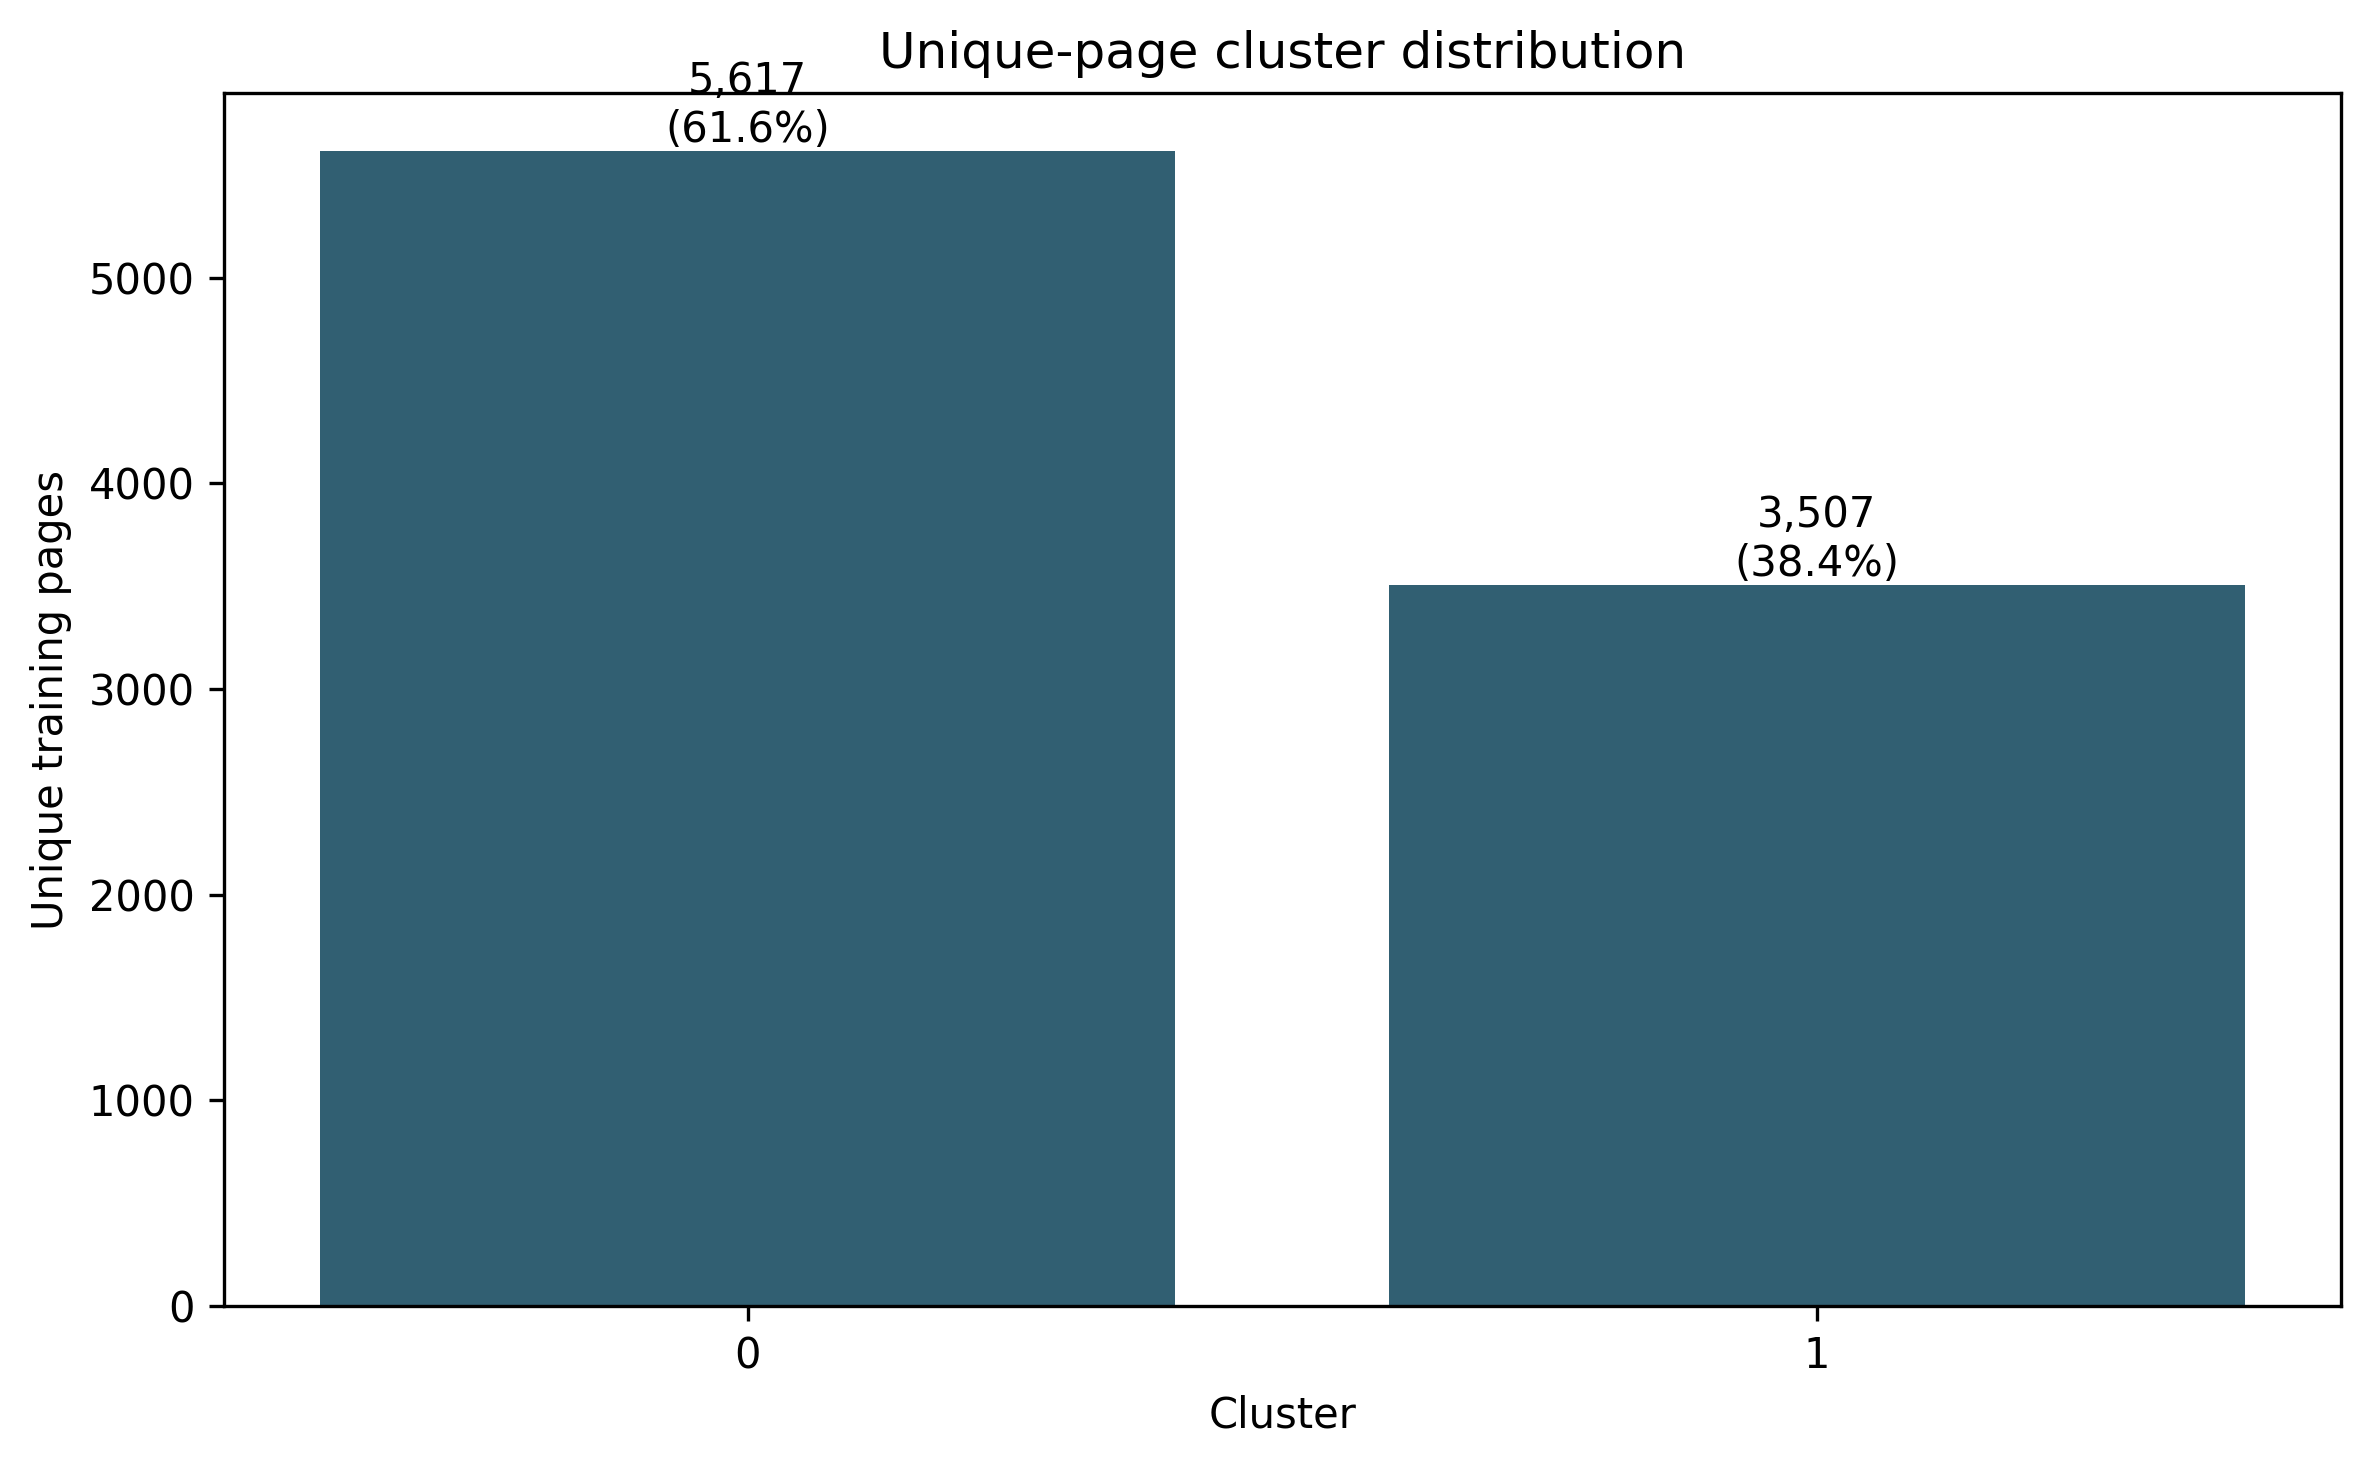
\includegraphics[width=0.75\textwidth]{figures/stage2/cluster_distribution.png}
    \caption{Stage 2 layout clustering: cluster size distribution for the chosen $k=2$.}
    \label{fig:stage2_cluster_dist}
\end{figure}

\begin{table}[H]
\centering
\caption{Layout cluster distribution for $k=2$ on annotated training pages}
\label{tab:clusters}
\begin{tabular}{@{}lrrr@{}}
\toprule
\textbf{Cluster} & \textbf{Samples} & \textbf{\%} & \textbf{Characteristics} \\ \midrule
0 & 8{,}935 & 34.8\% & Text-rich / dense layouts (mean $n_{\text{boxes}}\approx 25.36$) \\
1 & 16{,}757 & 65.2\% & Text-sparse / low-text layouts (mean $n_{\text{boxes}}\approx 0.062$) \\ \bottomrule
\end{tabular}
\end{table}

\subsection{PCA Visualization}
\label{subsec:pca}

Principal Component Analysis (PCA) \cite{pca} with two components explains 82.7\% of the variance (PC1: 71.8\%, PC2: 10.8\%). Figure~\ref{fig:stage2_pca} visualizes the separation between the two layout clusters.

\begin{figure}[H]
    \centering
    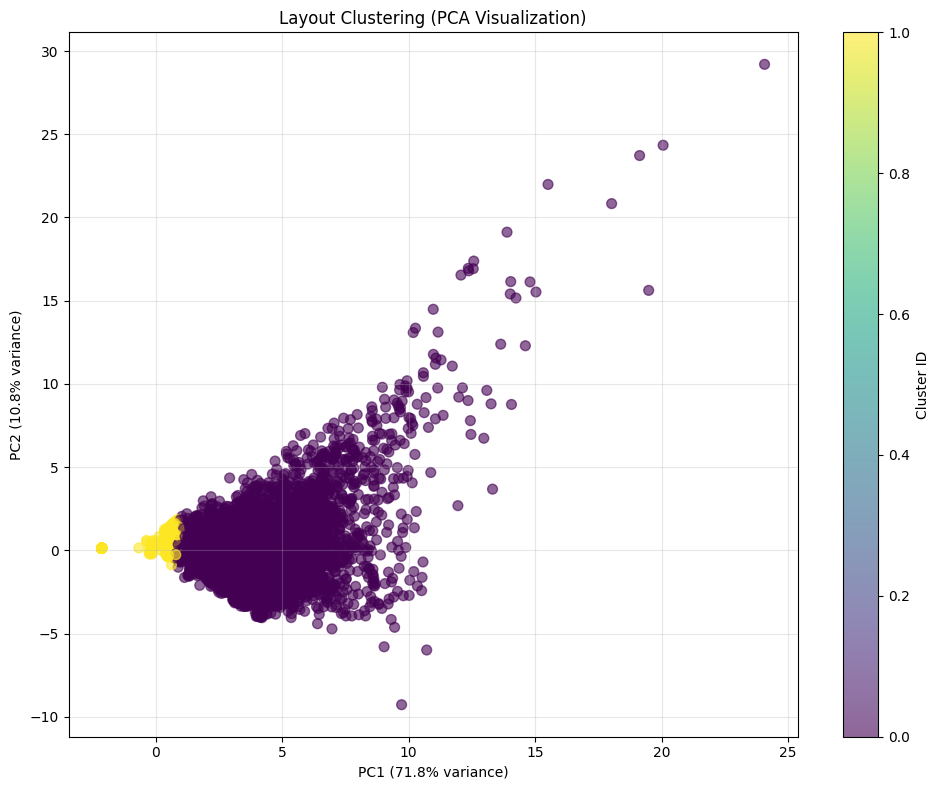
\includegraphics[width=0.80\textwidth]{figures/stage2/pca_clusters.png}
    \caption{PCA visualization of the $k=2$ layout clusters based on standardized layout features.}
    \label{fig:stage2_pca}
\end{figure}

As a qualitative robustness check, we also project the features with two
non-linear embeddings, t-SNE~\cite{tsne} and UMAP~\cite{umap}
(Figures~\ref{fig:stage2_tsne} and~\ref{fig:stage2_umap}). Unlike the linear PCA above (standardized
features), these projections apply a $\log(1+x)$ transform to the heavy-tailed
count/area features followed by robust scaling, and add a small Gaussian jitter
($\sigma=0.01$) so that the $\sim$16{,}757 identical empty-layout pages render as
a visible region rather than collapsing to a single point; t-SNE is computed on a
stratified 3{,}000-page subsample and UMAP on all 25{,}692 pages. They are
therefore exploratory visualizations rather than pixel-comparable to the PCA
plot, but all three consistently show the same two-way text-rich vs.\
text-sparse separation. The apparent internal spread of the sparse cluster is an
artifact of the added jitter (those pages share identical zero-valued features).

\begin{figure}[H]
    \centering
    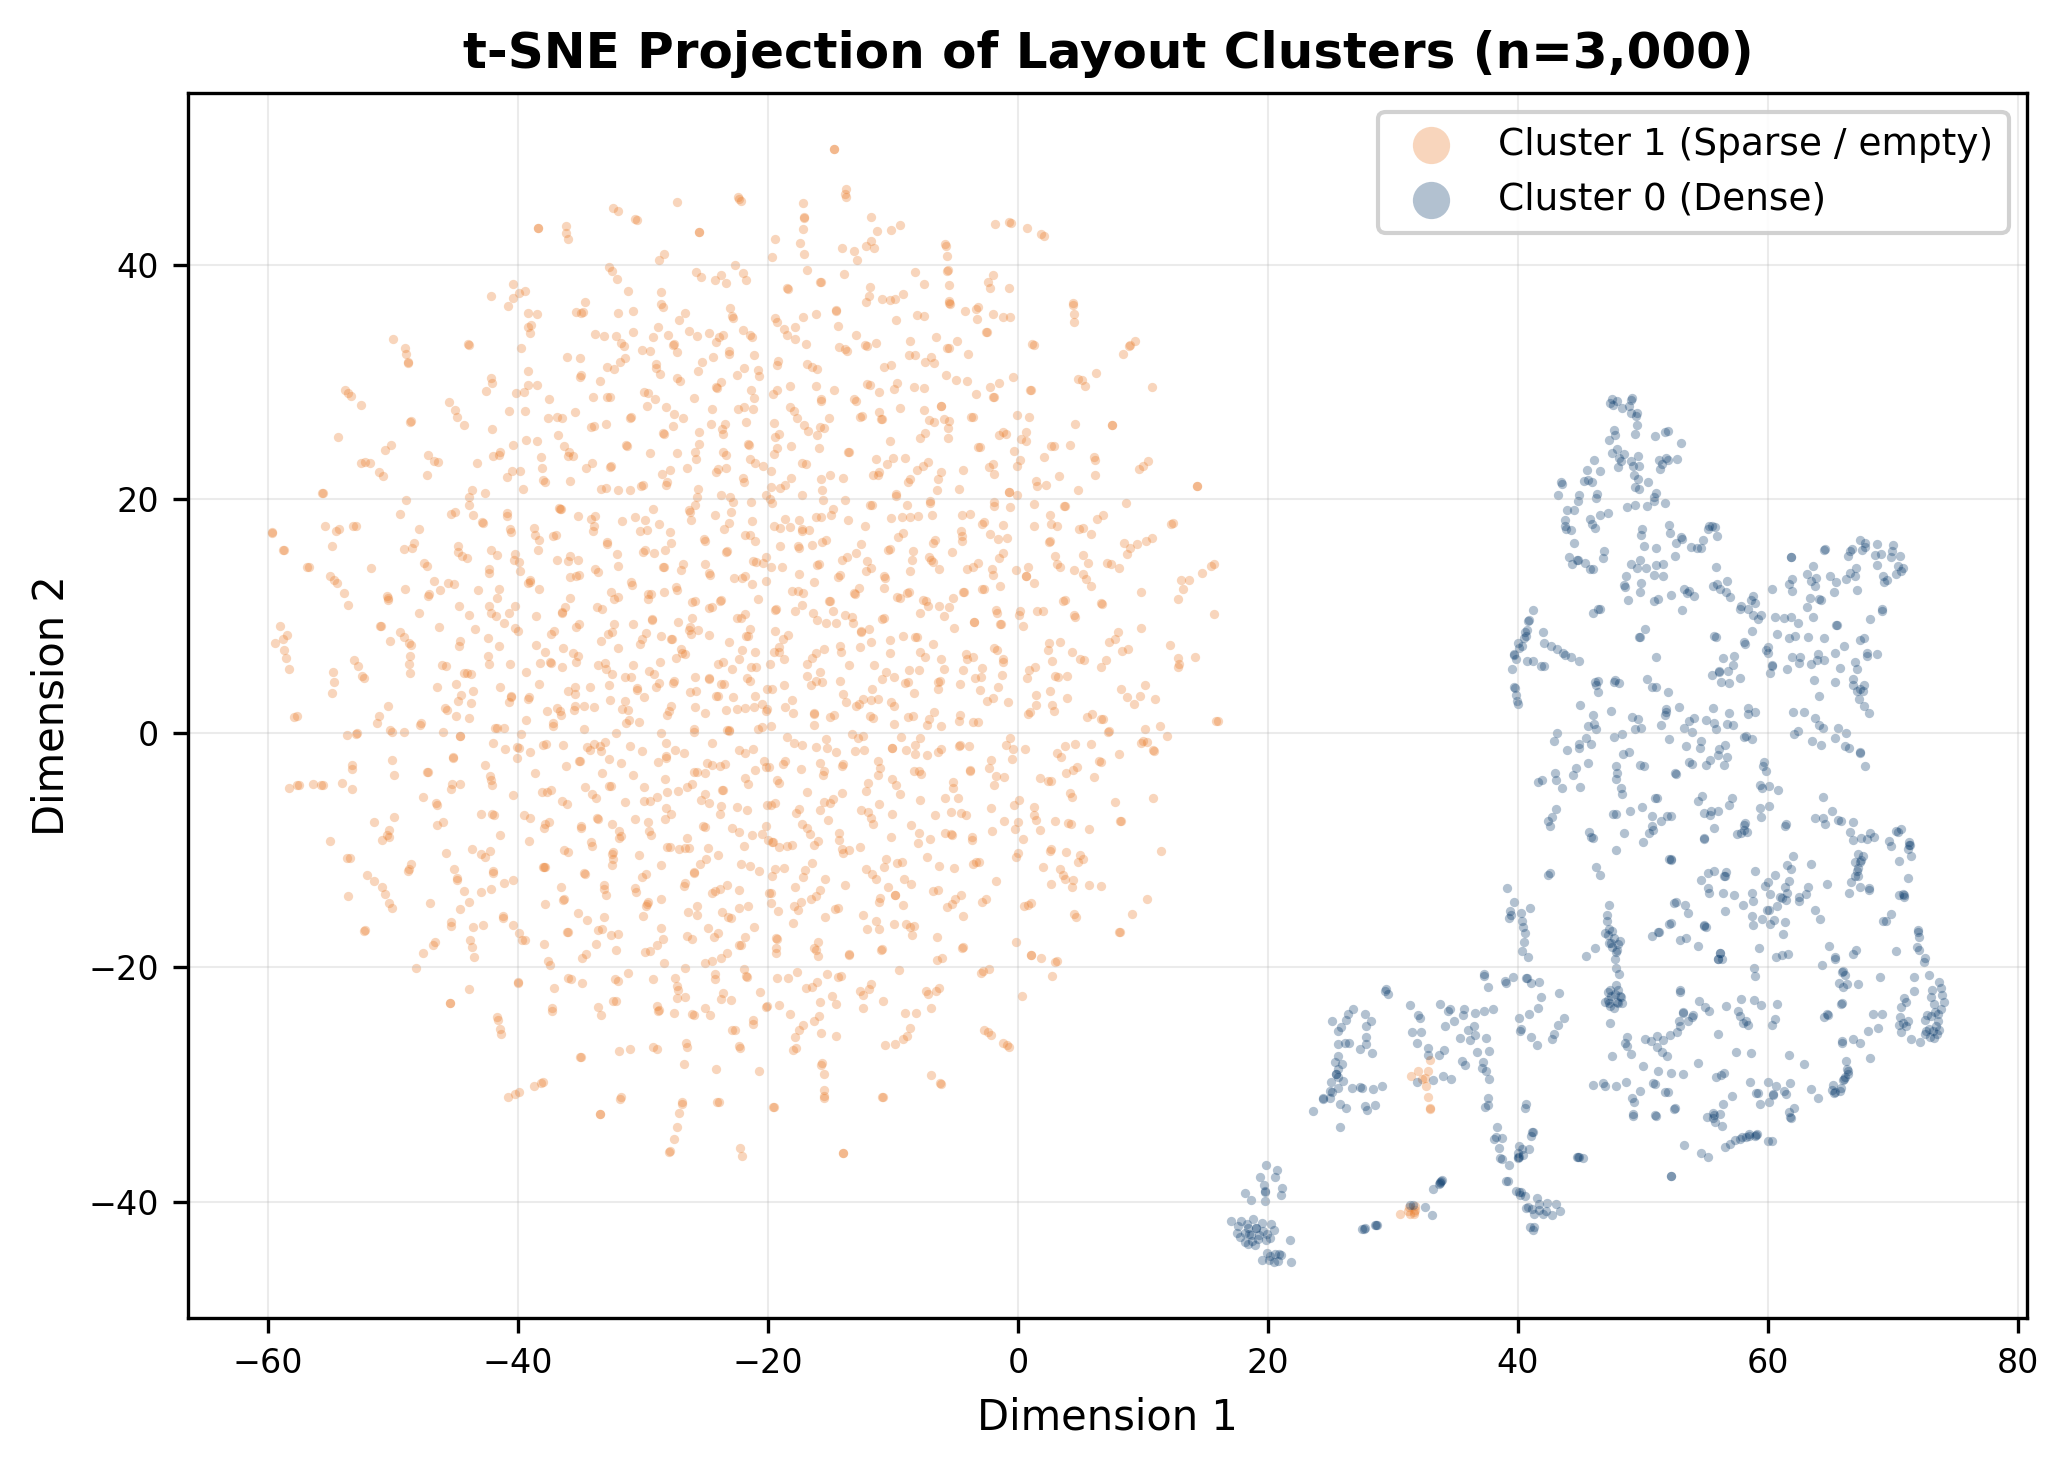
\includegraphics[width=0.72\textwidth]{figures/stage2/tsne_clusters.png}
    \caption{Non-linear t-SNE projection of the $k=2$ layout clusters, computed
    on a stratified 3{,}000-page subsample. Features are
    $\log(1+x)$-transformed, robust-scaled, and jittered ($\sigma=0.01$); the
    sparse cluster's spread is a jitter artifact, not real structure. It
    reproduces the separation observed in the PCA projection.}
    \label{fig:stage2_tsne}
\end{figure}

\begin{figure}[H]
    \centering
    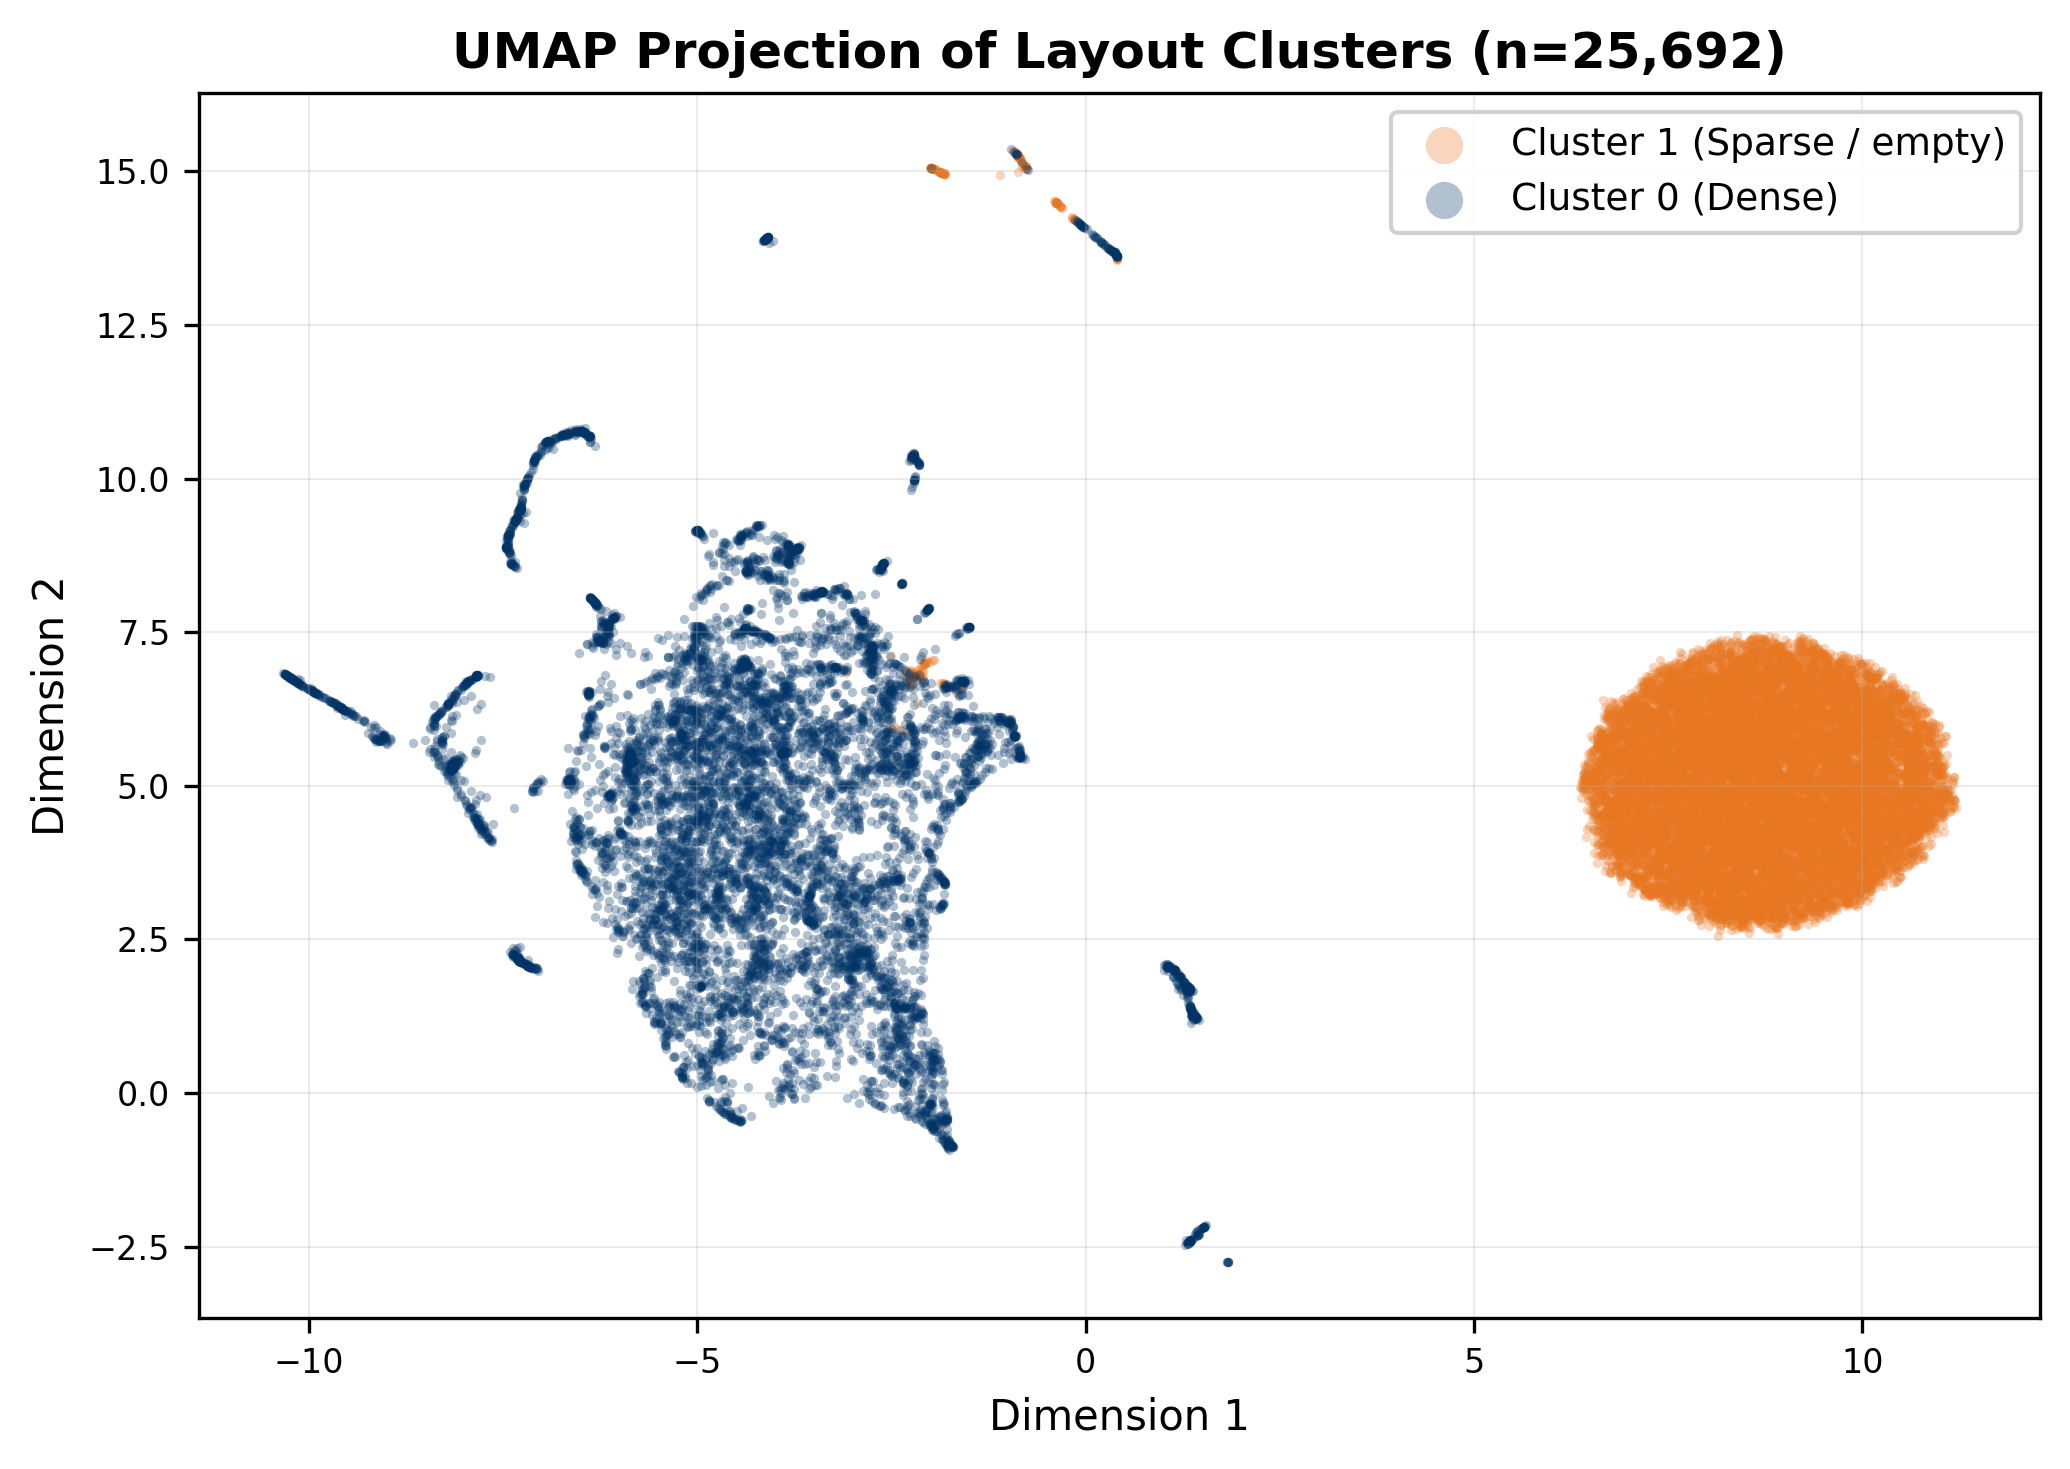
\includegraphics[width=0.72\textwidth]{figures/stage2/umap_clusters.png}
    \caption{Non-linear UMAP projection of the $k=2$ layout clusters, computed
    on all 25{,}692 pages with the same $\log(1+x)$ $+$ robust-scaling $+$
    jitter preprocessing as the t-SNE plot. It likewise reproduces the
    text-rich vs.\ text-sparse separation.}
    \label{fig:stage2_umap}
\end{figure}

To interpret the clusters, Figure~\ref{fig:stage2_feature_distributions} and Table~\ref{tab:stage2_cluster_stats} summarize how key layout statistics differ across clusters.

\begin{figure}[H]
    \centering
    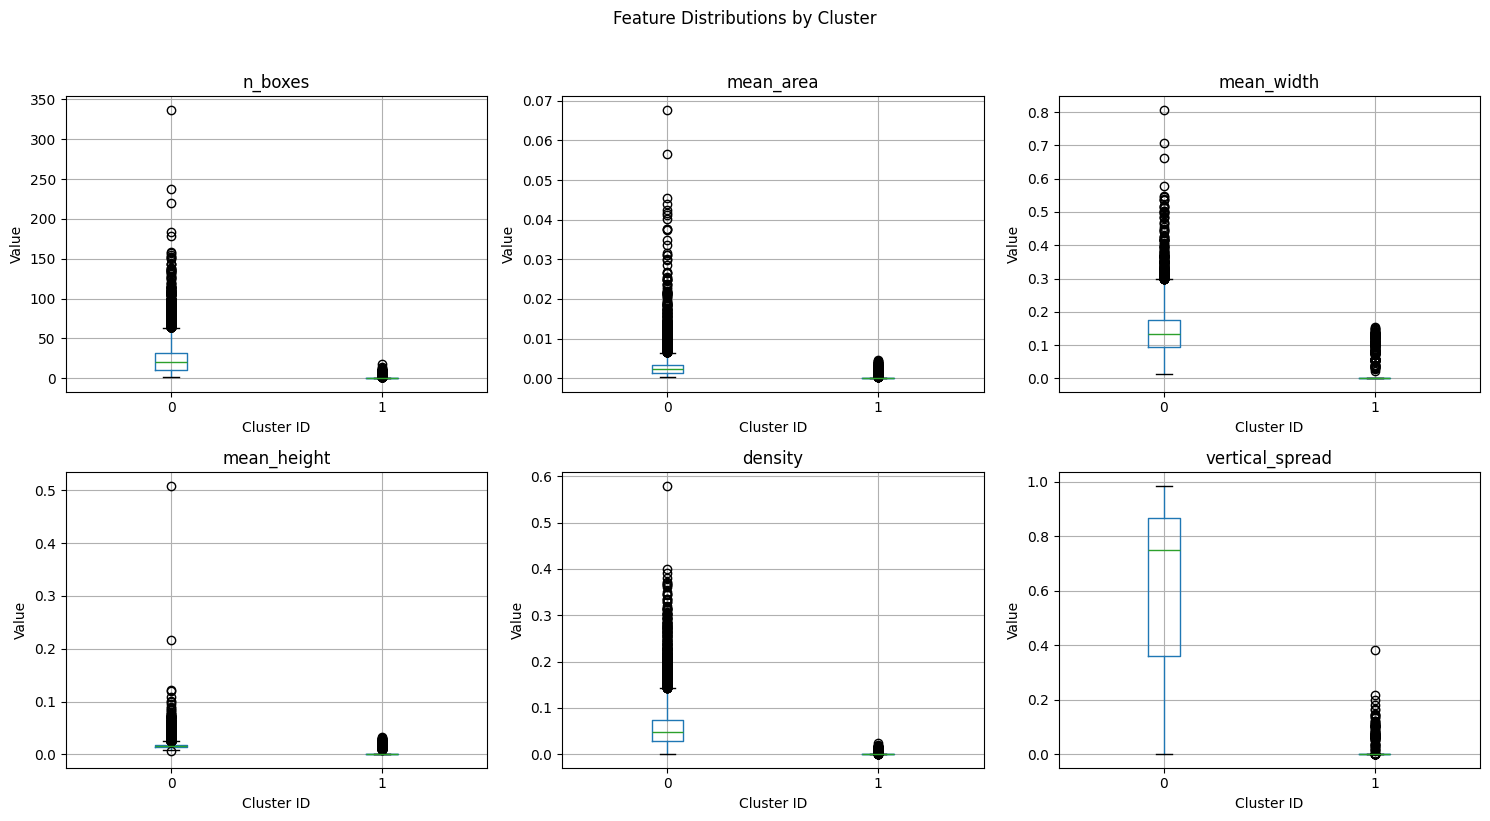
\includegraphics[width=0.90\textwidth]{figures/stage2/feature_distributions.png}
    \caption{Feature distributions by cluster for selected layout features (Stage 2).}
    \label{fig:stage2_feature_distributions}
\end{figure}

\begin{table}[H]
    \centering
    \small
    \caption{Summary statistics of selected layout features per cluster (mean\,$\pm$\,std).
    The page-coverage feature (total box area) is used as the layout density measure,
    so it is reported once.}
    \label{tab:stage2_cluster_stats}
    \begin{tabular}{@{}lrrr@{}}
        \toprule
        \textbf{Cluster}
            & \shortstack{\textbf{$n_{\text{boxes}}$}\\\textbf{mean $\pm$ std}}
            & \shortstack{\textbf{Coverage}\\\textbf{mean $\pm$ std}}
            & \shortstack{\textbf{Mean box area}\\\textbf{mean $\pm$ std}} \\
        \midrule
        0 (text-rich)   & $25.3622 \pm 20.5338$ & $0.0582 \pm 0.0467$ & $0.0029 \pm 0.0030$ \\
        1 (text-sparse) & $ 0.0619 \pm  0.6941$ & $0.0001 \pm 0.0009$ & $0.0000 \pm 0.0002$ \\
        \bottomrule
    \end{tabular}
\end{table}

The two principal components admit a clear interpretation. PC1 (71.8\% of the variance) captures overall content density --- the number of extractable text boxes and their coverage --- and this dominant axis is what separates the text-rich cluster from the text-sparse one. PC2 (10.8\%) captures secondary geometric variation beyond density.

\subsection{Use in Later Stages}
\label{subsec:cluster_use}

The scaler and $k$-means model are fitted on the annotated KVP10k training
pages described above. For later evaluation, this fitted model is kept fixed:
features are computed for each test page, transformed by the training-fitted
scaler, and assigned to the nearest learned cluster. Thus, cluster discovery
uses the training split, while the per-cluster performance reported in
Stages~3--4 is measured on the held-out test set (see
Section~\ref{sec:stage3-per-cluster}).

\section{Key-Value Link Analysis}
\label{sec:kv_analysis}

We analyze spatial relationships between linked \kvps{} to inform model design.

\subsection{Spatial Proximity}

For each key-value pair with linking annotation, we compute the Euclidean distance between bounding box centers:

\begin{equation}
d_{kv} = \sqrt{(x_v - x_k)^2 + (y_v - y_k)^2}
\end{equation}

where $(x_k, y_k)$ and $(x_v, y_v)$ are the normalized center coordinates of the key and value boxes.

On a 200-sample subset containing 755 links,\footnote{This 200-page subset is the manually inspected annotation subsample used for the spatial analysis; it is distinct from the 581-page evaluation test set (3{,}776 ground-truth links) reported in Chapter~\ref{ch:exresults}. The two figures refer to different data slices, not conflicting counts of the same set.} linked pairs are strongly proximate: the mean key--value distance is $\mu_d = 0.10$, the median is $\tilde{d} = 0.08$, and the 90th percentile is $d_{90} = 0.15$ (all in normalized units). Since most \kvps{} lie within 0.15 normalized units of each other, spatial features are clearly informative for accurate linking.

\section{Annotation Statistics}
\label{sec:annotation_stats}

\begin{table}[h]
\centering
\caption{Annotation statistics for 200-sample subset}
\label{tab:ann_stats}
\begin{tabular}{@{}lr@{}}
\toprule
\textbf{Metric} & \textbf{Value} \\ \midrule
Total samples & 200 \\
Samples with annotations & 200 (100\%) \\
Total annotations & 7,000+ \\
Mean annotations per sample & $\sim$35 \\
Annotations with linking & 755 \\
Percentage with linking & $\sim$60\% \\ \bottomrule
\end{tabular}
\end{table}

\section{Summary}
\label{sec:dataset_summary}

The dataset analysis yields four main observations: the annotated pages fall into two distinct layout types of differing text density; linked \kvps{} are strongly spatially proximate; the annotations are of high quality with consistent linking information; and two principal components already capture 82.7\% of the layout-feature variance. These insights inform our model design, particularly the importance of spatial encoding in the linker module.
